%-------------------------------------------------------------------------------
% 32-chapter-two.tex
%
% Материалы и методы исследования
%
% Автор шаблона: Гордеев Иван
%-------------------------------------------------------------------------------

\section{Материалы и методы исследования}
\label{ch:methods}

\subsection{Рентгеновская установка}

В данной работе интерес представляют дозиметрические характеристики излучения рентгеновской трубки установки CellRad (см. Рис.~\ref{img:CellRad}). Характеристики определялись путем моделирования. Основные параметры установки приведены в Таблице~\ref{tab:parameters}.

\begin{figure}[!htb]
\begin{minipage}{0.5\linewidth}
\center
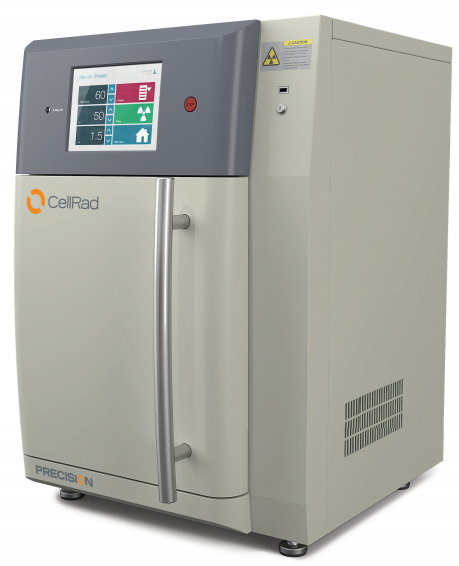
\includegraphics[width=0.9\linewidth]{img/CellRad}
\end{minipage}
% \hfill
\begin{minipage}{0.5\linewidth}
\center
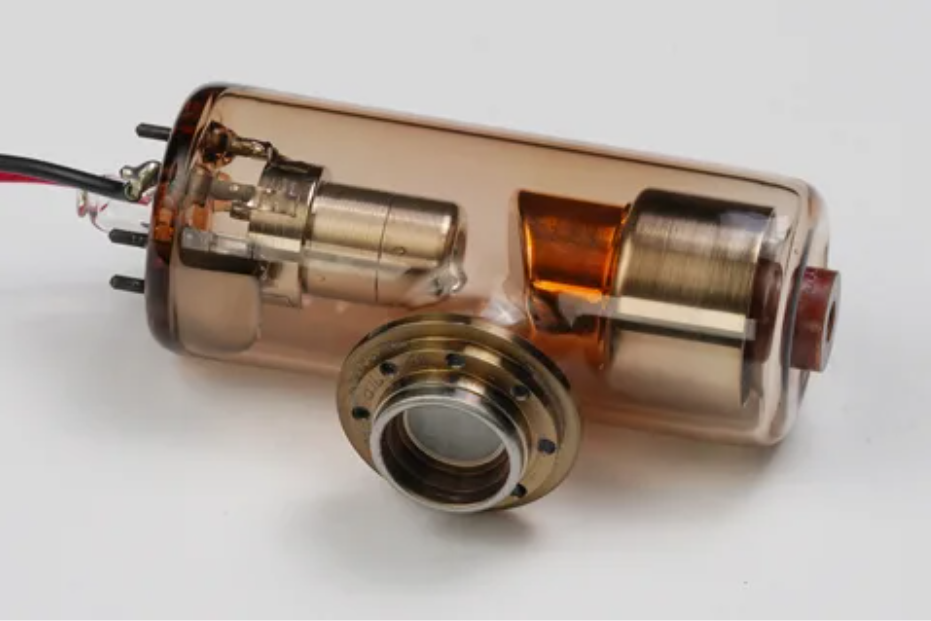
\includegraphics[width=1\linewidth]{img/XRayTube}
\end{minipage}
\vspace{5mm}
\caption{Установка CellRad фирмы Precision (слева), тип рентгеновской трубки (справа)}
\label{img:CellRad}
\end{figure}


\begin{table}[h]
\centering
\begin{tabular}{|c|c|c|c|}\hline
Макс. напряжение, кВ & Угол наклона анода, \textdegree  & Материал мишени & Внешняя фильтрация \\\hline
130 & 20 & W & 0.5 мм Al  \\\hline
\end{tabular}
\caption{Параметры рентгеновской трубки установки CellRad}
\label{tab:parameters}
\end{table}


Для расчета поглощенной дозы необходимо:
\begin{enumerate}[topsep=0pt,itemsep=-1ex,partopsep=1ex,parsep=1ex]
    \item Найти распределение флюенса по глубине проникновения в среду/материал. 
    \item Найти взвешенный по энергии флюенс.
    \item Найти значения массового коэффициента для всех соответствующих значений флюенса.
    \item Определить керму по формуле для каждого слоя.
    \item Определить глубину, на которой наблюдается электронное равновесие. С этой глубины можно считать, что поглощенная доза равна керме.
\end{enumerate} 
